\documentclass[fleqn]{article}
\usepackage{amsmath}
\usepackage{amssymb}
\usepackage{enumitem}  
\usepackage{graphicx}
\usepackage[a4paper,margin=0.5in,footskip=0.15in]{geometry}

\date{\today}
\author{Ali Abbas}
\title{70103 Statistical Information Theory CW}

\begin{document}
  \maketitle
  \section{Analytic Comparison}
  The probability of correctly decoding a Hamming code with $n = 2^m - 1$ bits can be decomposed as such:
  \begin{align*}
    P_{\text{correct}} = P_{\text{no error}} + P_{\text{single bit flip}}
  \end{align*}
  
  The probability of no errors is:
  \begin{align*}
    P_{\text{no error}} = (1 - p)^n
  \end{align*}
  
  The probability of exactly one bit flipping is:
  \begin{align*}
    P_{\text{single bit flip}} = \binom{n}{1} \cdot p \cdot (1 - p)^{n-1}
  \end{align*}
  
  And so:
  \begin{align*}
    P_{\text{correct}} &=\ (1 - p)^n + \binom{n}{1} \cdot p \cdot (1 - p)^{n-1} \\
     &=\ (1 - p)^n \cdot \left(1 + \cdot \frac{n \cdot p}{1 - p}\right)
  \end{align*}

  Therefore, for a completely noise ($p = 0.5$) binary symmetric channel, for $m \in \{2, 3, 4 \}$ we have:
  \begin{align*}
    m = 2: P_{\text{correct}} &= 0.5 \\
    m = 3: P_{\text{correct}} &= 0.0625 \\
    m = 4: P_{\text{correct}} &= 0.00048828125
  \end{align*}
  And the numerical results are similar:
  \begin{align*}
    m = 2: P_{\text{correct numerical}} &= 0.485 \\
    m = 3: P_{\text{correct numerical}} &= 0.066 \\
    m = 4: P_{\text{correct numerical}} &= 0.0
  \end{align*}

  \pagebreak

  \section{Visual Comparison}
  In this section there are 3 plots which show the decoder accuracy vs the noise probability for $m \in \{ 2, 3, 4 \}$, as well as a final combined plot to visualise the differences between various $m$.
  \begin{figure}[ht!]
      \centering
      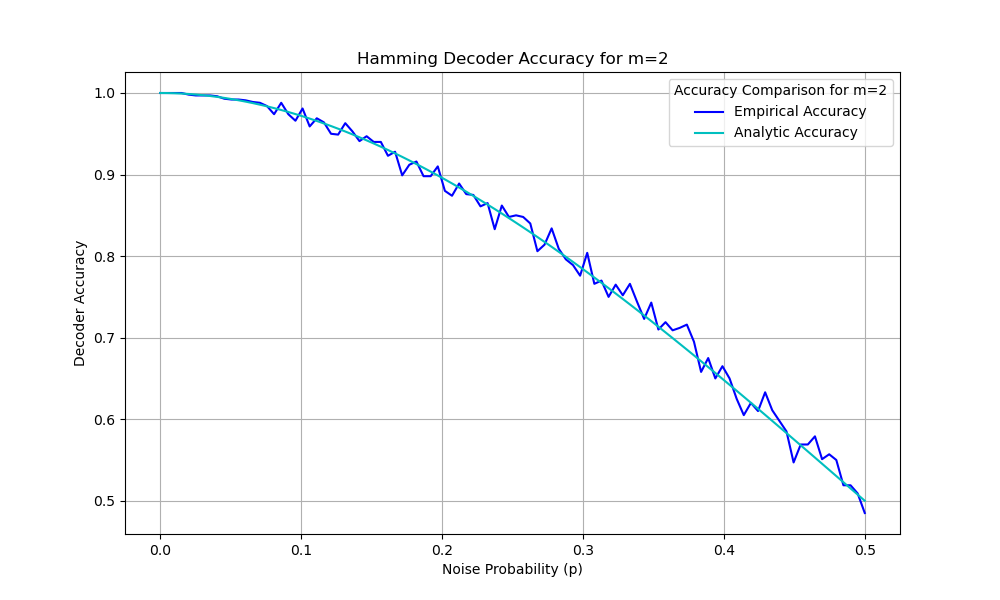
\includegraphics[width=1.0\textwidth]{../images/accuracy_m2.png}
      \caption{Hamming Decoder Accuracy for $m=2$}
      \label{fig:accuracy_m2}
  \end{figure}

  \begin{figure}[ht!]
      \centering
      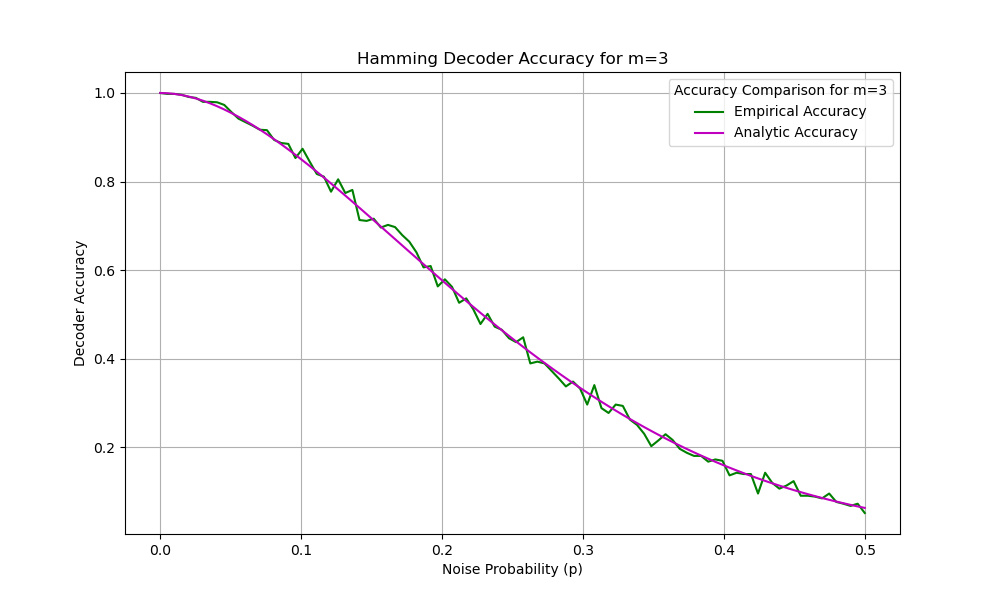
\includegraphics[width=1.0\textwidth]{../images/accuracy_m3.png}
      \caption{Hamming Decoder Accuracy for $m=3$}
      \label{fig:accuracy_m3}
  \end{figure}
  
  \begin{figure}[ht!]
      \centering
      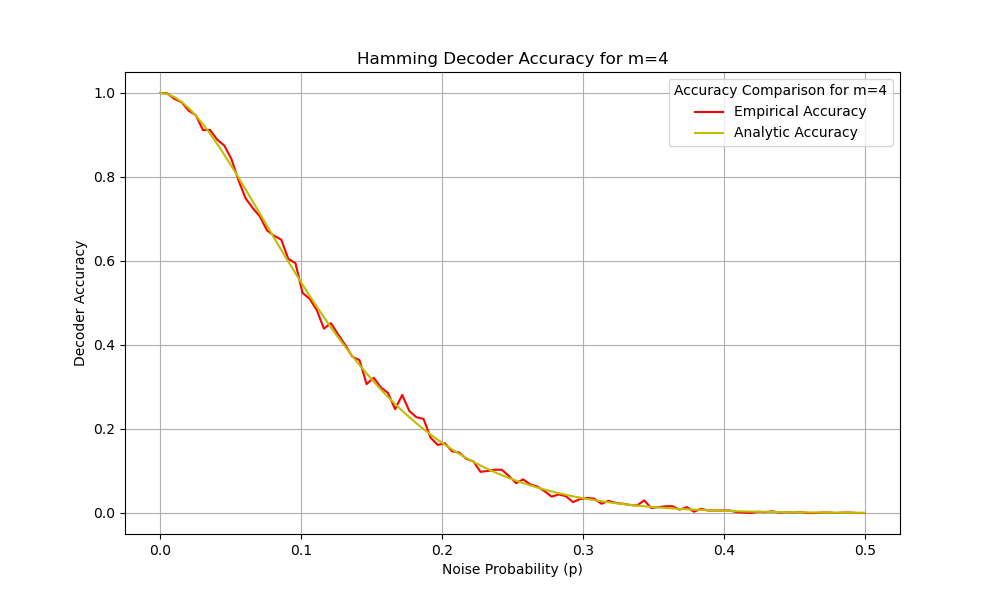
\includegraphics[width=1.0\textwidth]{../images/accuracy_m4.png}
      \caption{Hamming Decoder Accuracy for $m=4$}
      \label{fig:accuracy_m4}
  \end{figure}

  \begin{figure}[ht!]
      \centering
      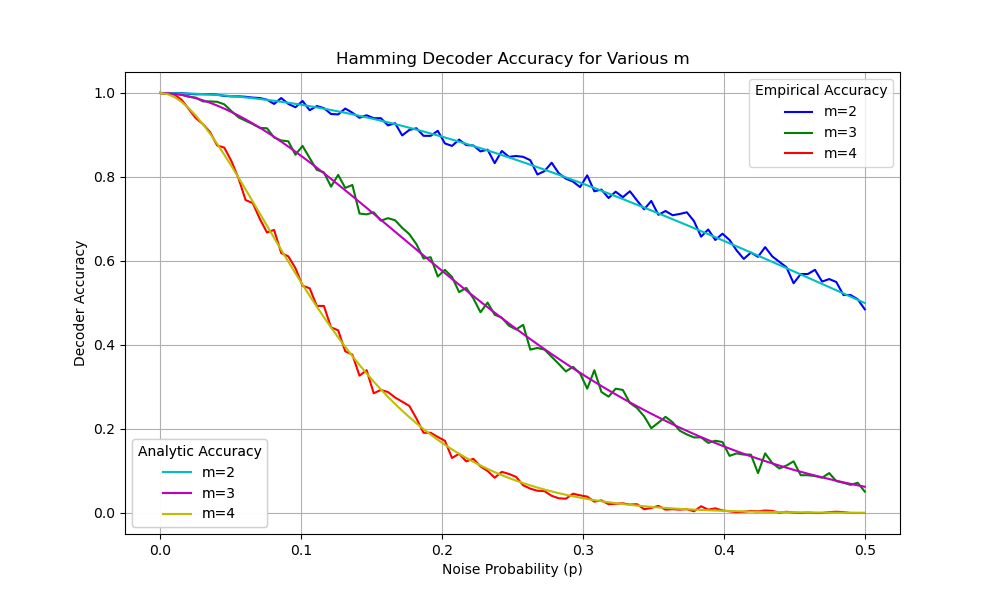
\includegraphics[width=1.0\textwidth]{../images/accuracy_overlay.png}
      \caption{Hamming Decoder Accuracy for $m \in \{ 2, 3, 4 \}$}
      \label{fig:accuracy_overlay}
  \end{figure}

  From these figures, I conclude that Hamming codes perform well for low noise settings, but their error correcting abilities are impacted as noise increases (since Hamming codes can't correct multiple bit errors).
  For subsequently higher values of $m$ (and thus for longer codewords) the rate of dropoff in performance increases considerably, highlighting that they aren't suitable for correcting multiple bit errors.
  The dropoff in performance is intuitively due to the decreased proportion of error correcting bits relative to data bits for higher values of $m$, which reduces the redundancy of the code.
\end{document}
